%alex
\section{Trafic routier}
\subsection{Pr\'esentation}
\begin{frame}{Exemple 1 : \og trafic routier \fg{}}
Ici $E = [\![0, 2^{n}-1]\!]$. Pour tout $x\in E$, on note $x_i$ l'$(i+1)$-\`eme chiffre de l'\'ecriture de $x$ en base $2$.
\[\begin{array}{ccc}
x_{\scriptscriptstyle i+1}x_{\scriptscriptstyle i}x_{\scriptscriptstyle i-1} & & f(x)_i\\
?11 & \mapsto & 1\\
?10 & \mapsto & 0\\
10? & \mapsto & 1\\
00? & \mapsto & 0\\
\end{array}\]
\end{frame}

\begin{frame}
Avec $n=5$ et $x=21$:
\[\begin{array}{cc}
p & f^{p}(x)\\
0 & 10101\\
1 & 01011\\
2 & 10110\\
3 & 01101\\
\end{array}\]
\end{frame}

\subsection{Algorithmes}
\begin{frame}
\begin{figure}
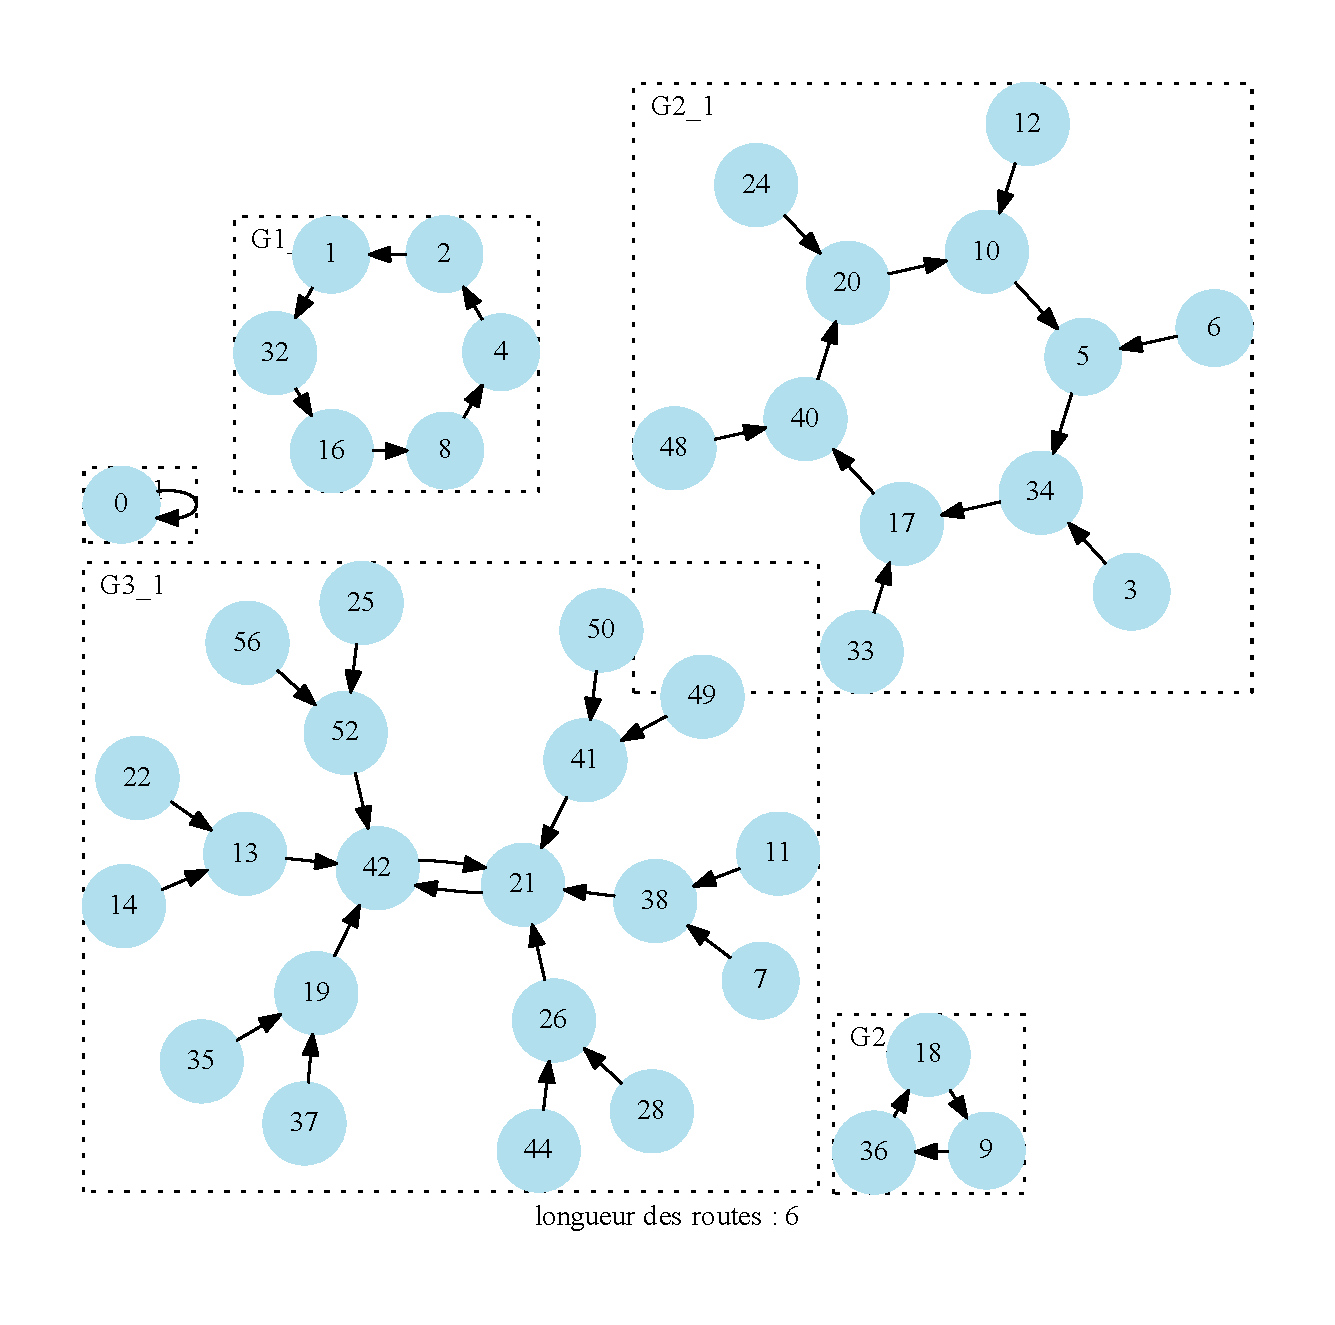
\includegraphics[scale=0.35]{./images/graph_6}
\caption{quelques composantes connexes de $G_f$ pour $n=6$}
\end{figure}
\end{frame}

\begin{frame}{Algorithme}
\begin{algorithm}[H]
\SetKwInOut{Input}{Entr\'ee}
\SetKwInOut{Output}{Sortie}
\SetKwInOut{Var}{Variables}
\Input{$L$ : liste des \'el\'ements de $E$, ensemble fini\\$f$ : application de $E$ dans $E$}
\Output{le graphe $G_f$}
\Var{$R$ : liste courante constitu\'ee d'\'el\'ements de $E$\\$i$ : entier\\$P$ : tableau contenant les positions des \'el\'ements de $E$ dans le graphe (les cases de $P$ ne sont pas initialis\'ees et $L[j]$ correspond \`a $P[j]$ pour tout $j$ dans $[\![0, 2^{n}-1]\!]$)}
\end{algorithm}
\end{frame}

\begin{frame}{Algorithme}
\begin{algorithm}[H]
\SetKwBlock{Do}{It\'erer}{Boucler}\fontsize{8}{6}\selectfont
\Tq{$L$ contient un \'el\'ement $e_0$ de $E$ avec $L[i_0]=e_0$ et $P[i_0]$ n'est pas initialis\'ee}{
$i\leftarrow 0$\;
$R[0]\leftarrow e_0$\;
\Do{
$e\leftarrow f(R[i])$\;
\eSi{$e$ existe dans $R$}{
r\'ecup\'erer son index $i_e$ dans $R$\;
\eSi{$i_{e}=0$}{
ajouter le circuit $R$ au graphe\;
}{
ajouter le chemin $R[0, i_{e}]$ et le circuit $R[i_{e}, i]$ au graphe\;
}
initialiser les \'el\'ements de $P$ correspondant \`a ceux de $R$\;
sortir de la boucle\;
}{
trouver l'index $i_{L}(e)$ de $e$ dans $L$\;
$i\leftarrow i+1$\;
$R[i]\leftarrow e$\;
\Si{$P[i_{L}(e)]$ est initialis\'ee}{
ajouter le chemin $R[0, i]$ au graphe\;
mettre \`a jour les cases de $P$\;
sortir de la boucle\;
}
}
}
}
\end{algorithm}
\end{frame}

\begin{frame}
\begin{figure}
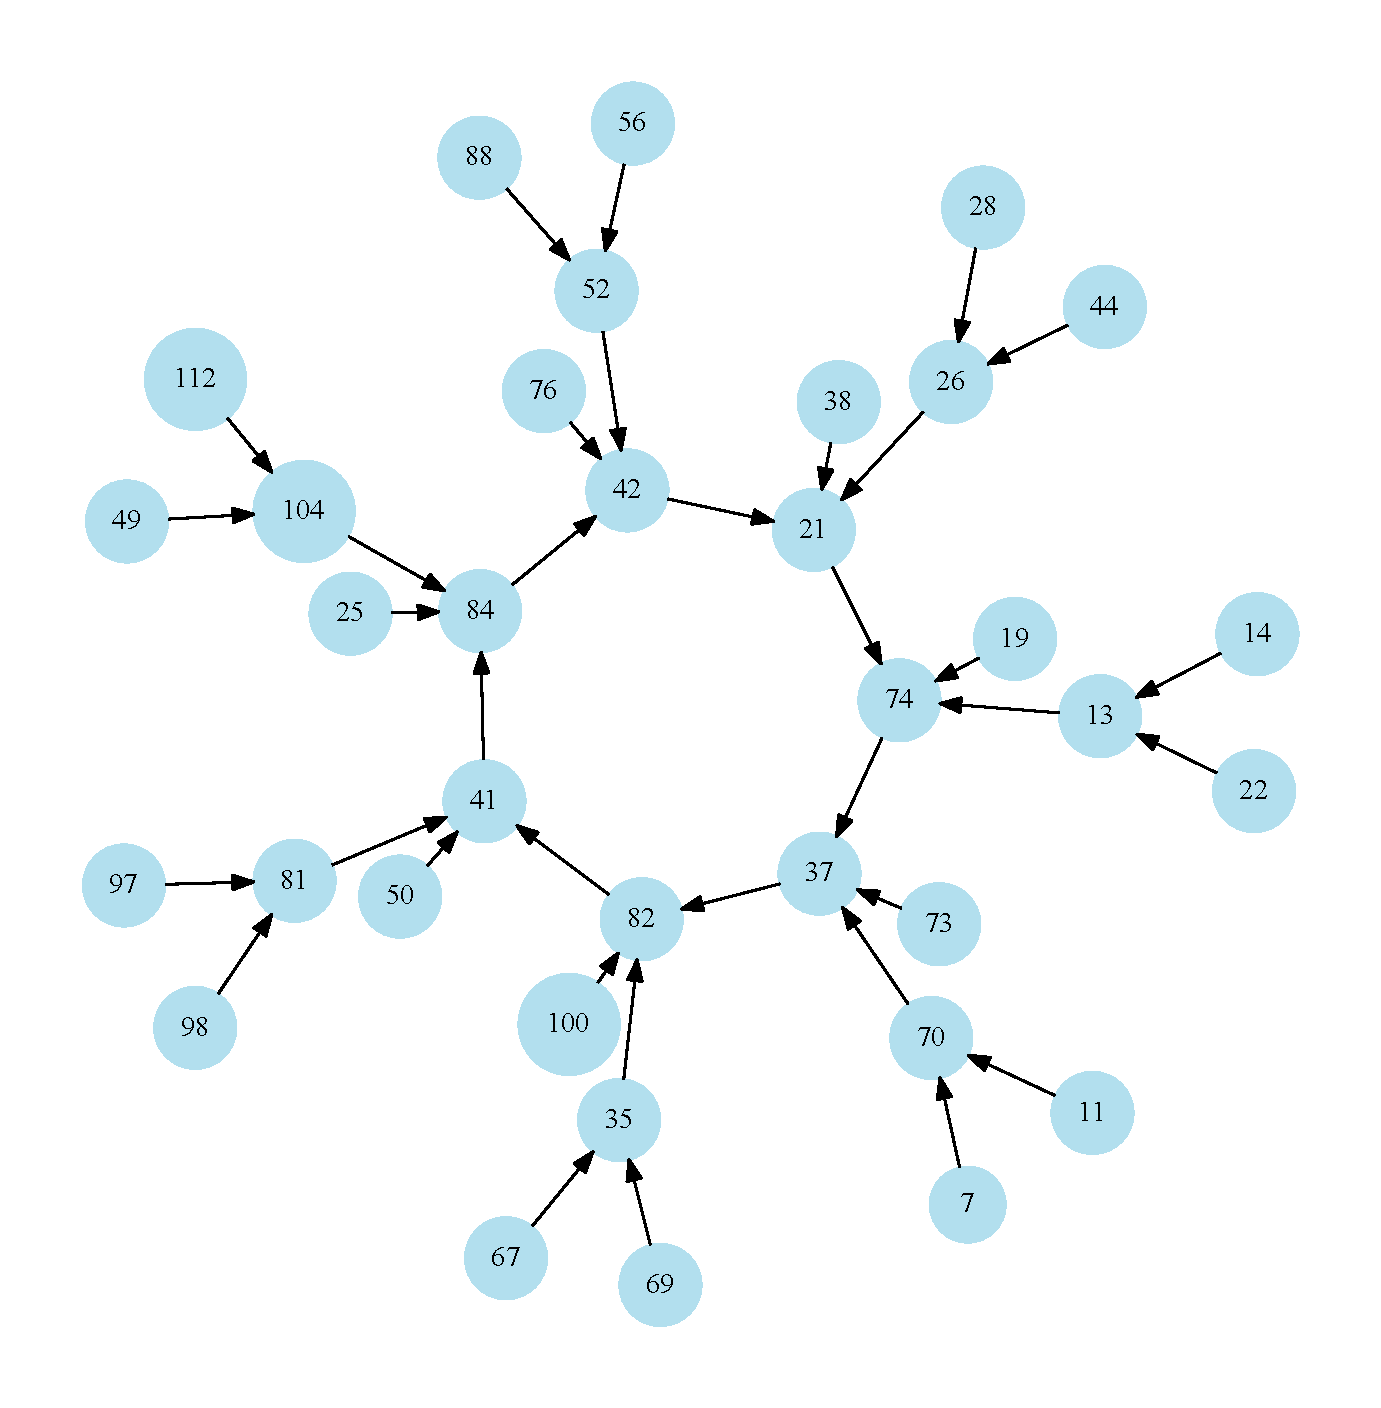
\includegraphics[scale=0.33]{./images/graph}
\caption{une composante connexe de $G_f$ lorsque $n=7$}
\end{figure}
\end{frame}

\begin{frame}
\begin{figure}
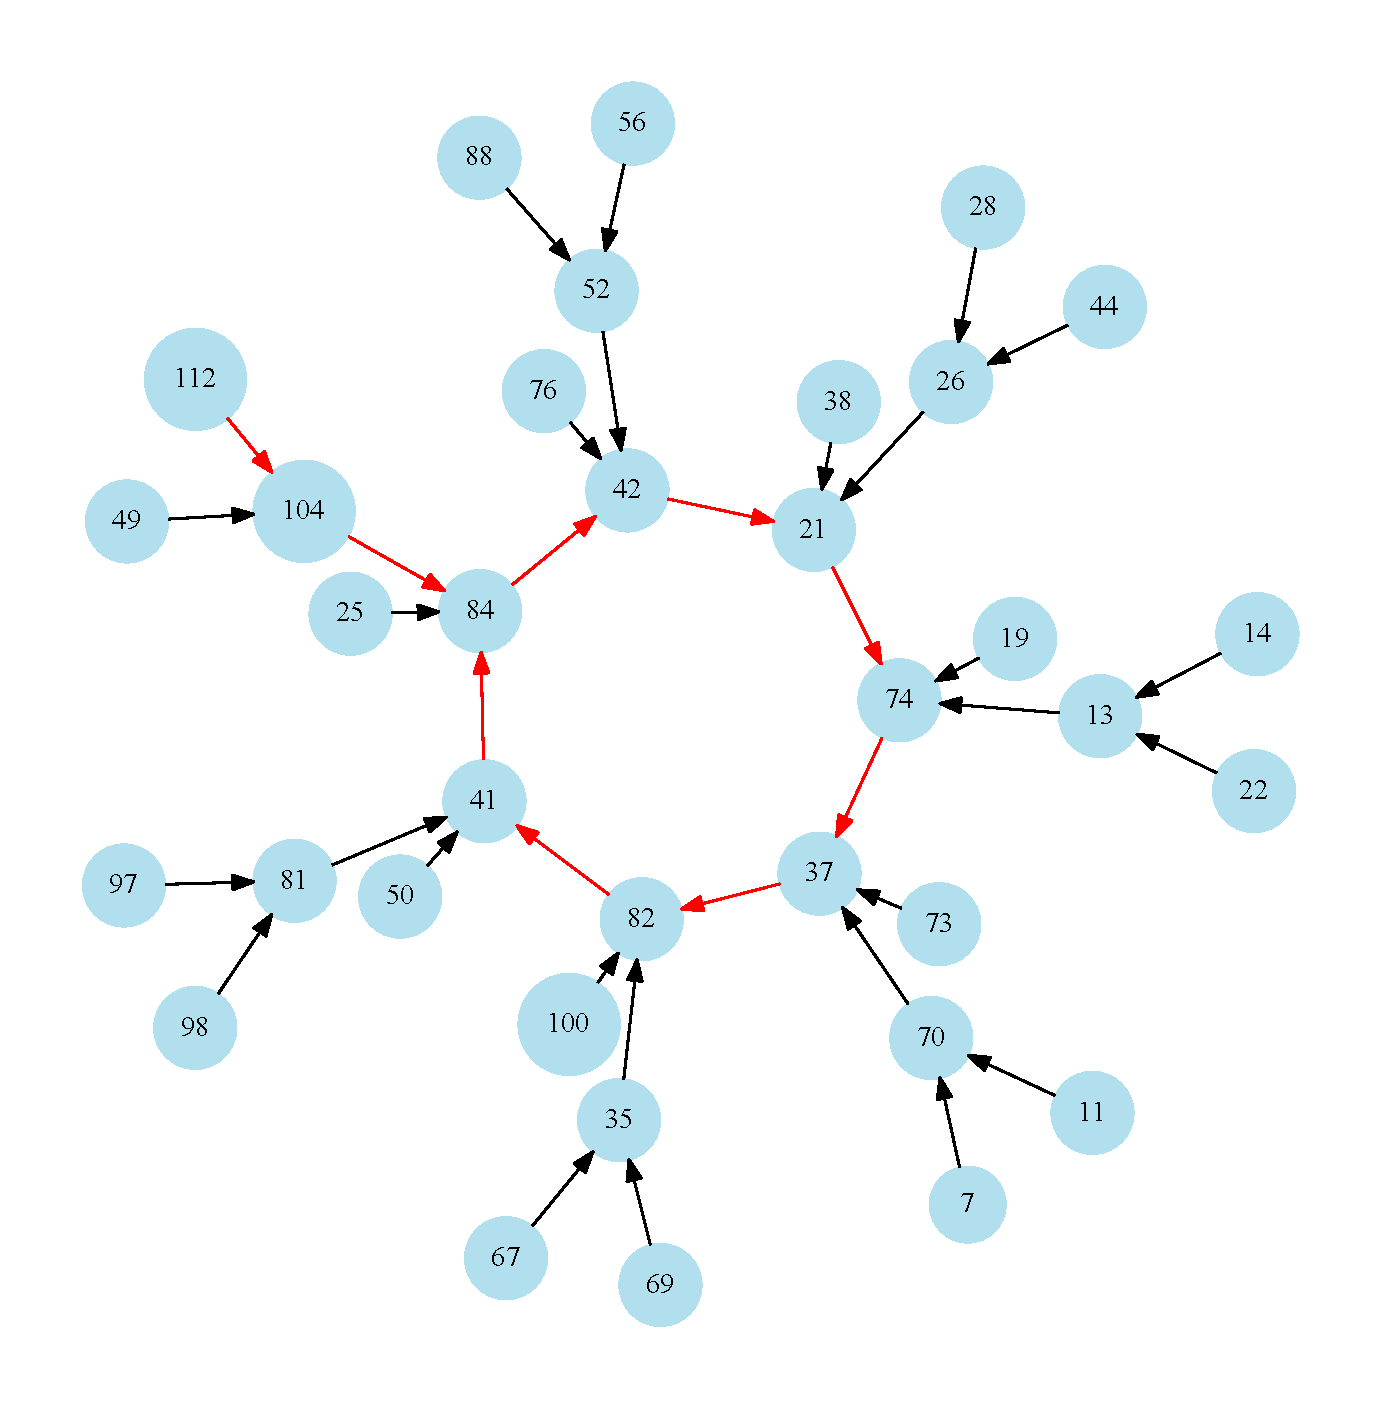
\includegraphics[scale=0.33]{./images/graph2}
\caption{\textcolor{red}{$9$} premi\`eres it\'erations}
\end{figure}
\end{frame}

\begin{frame}
\begin{figure}
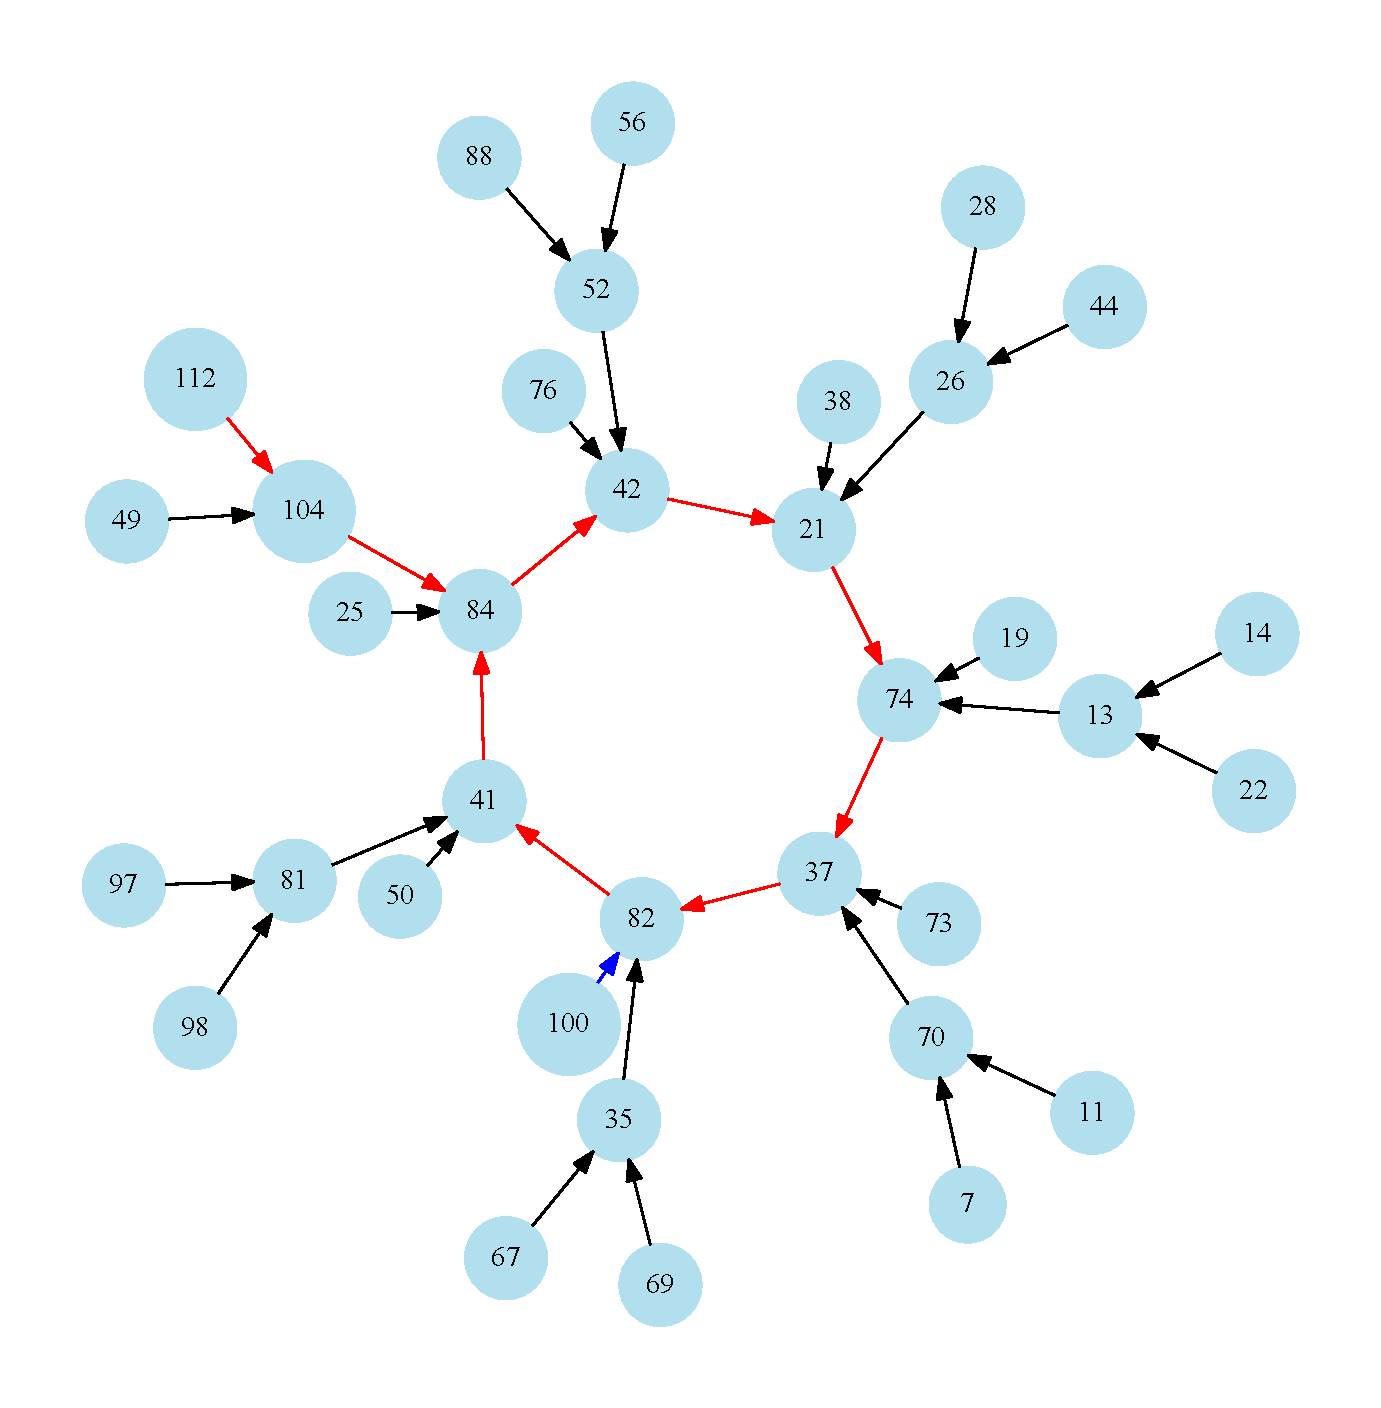
\includegraphics[scale=0.33]{./images/graph3}
\caption{\textcolor{blue}{$10$} premi\`eres it\'erations}
\end{figure}
\end{frame}

\begin{frame}
\begin{figure}
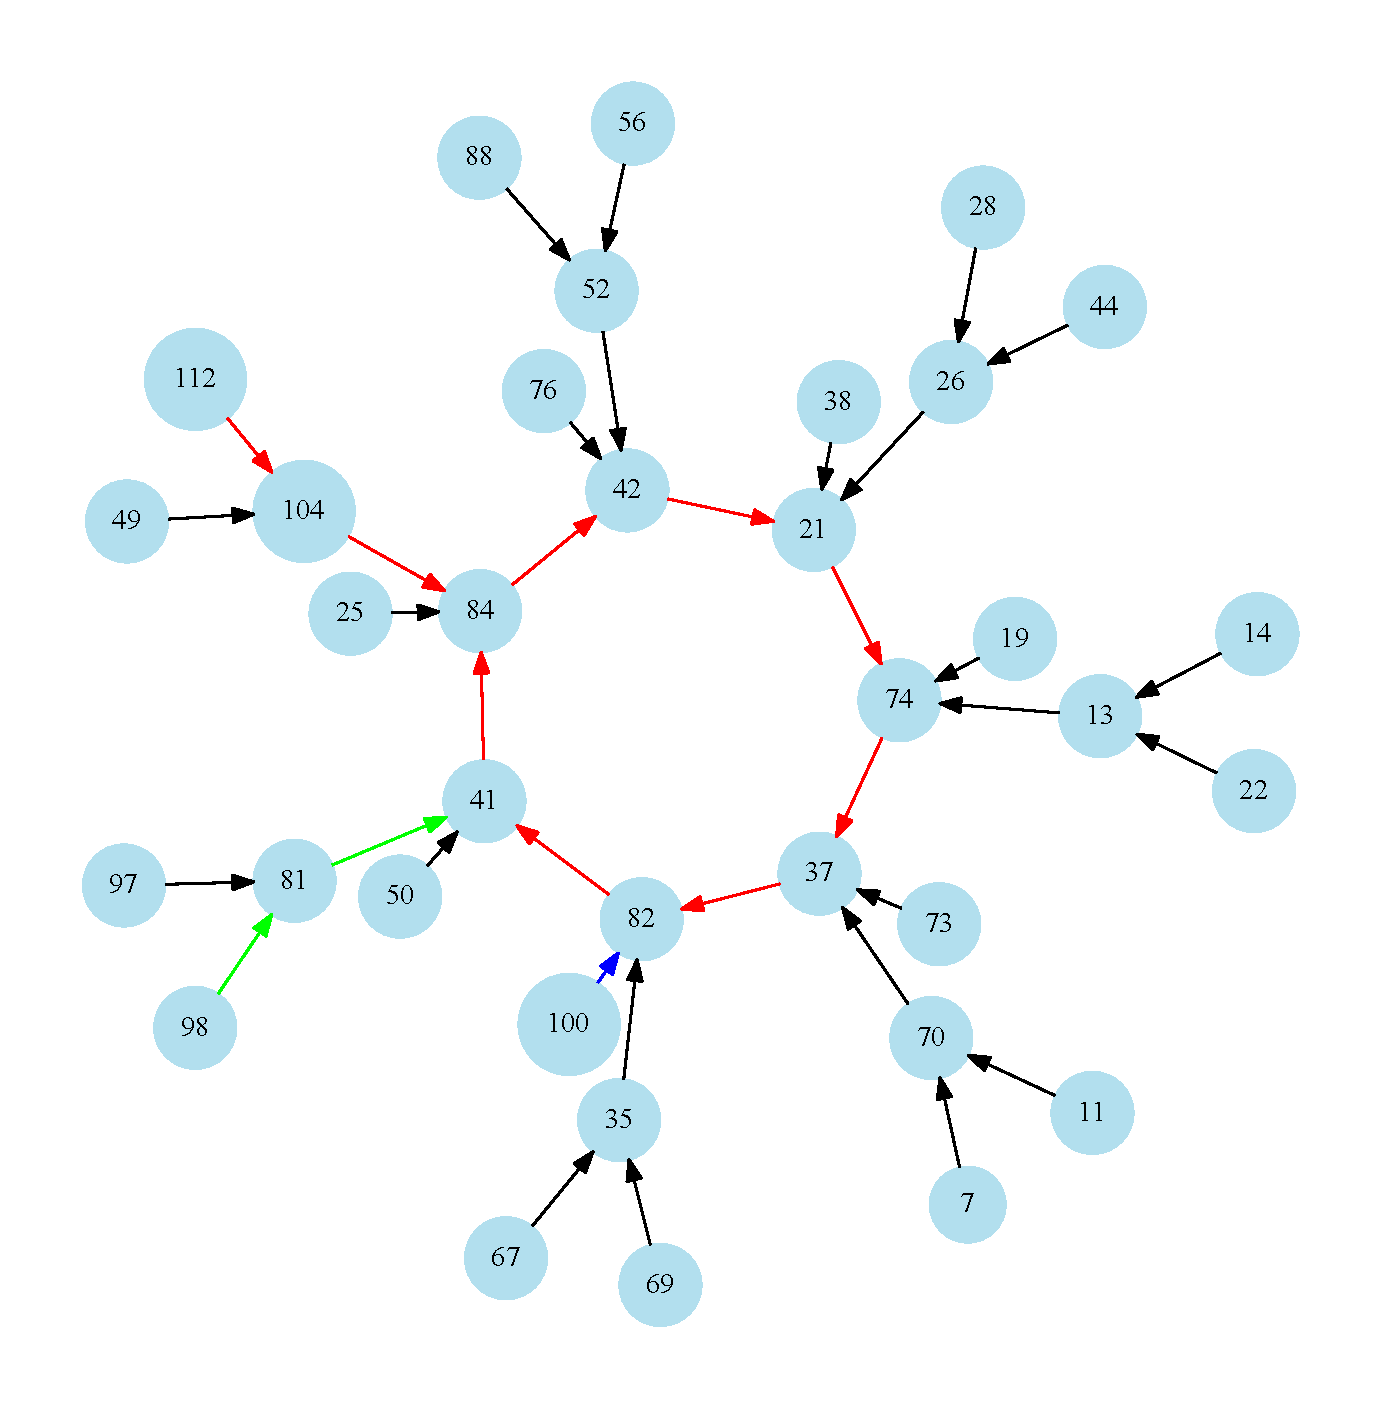
\includegraphics[scale=0.33]{./images/graph4}
\caption{\textcolor{green}{$12$} premi\`eres it\'erations}
\end{figure}
\end{frame}

\begin{frame}
\begin{figure}
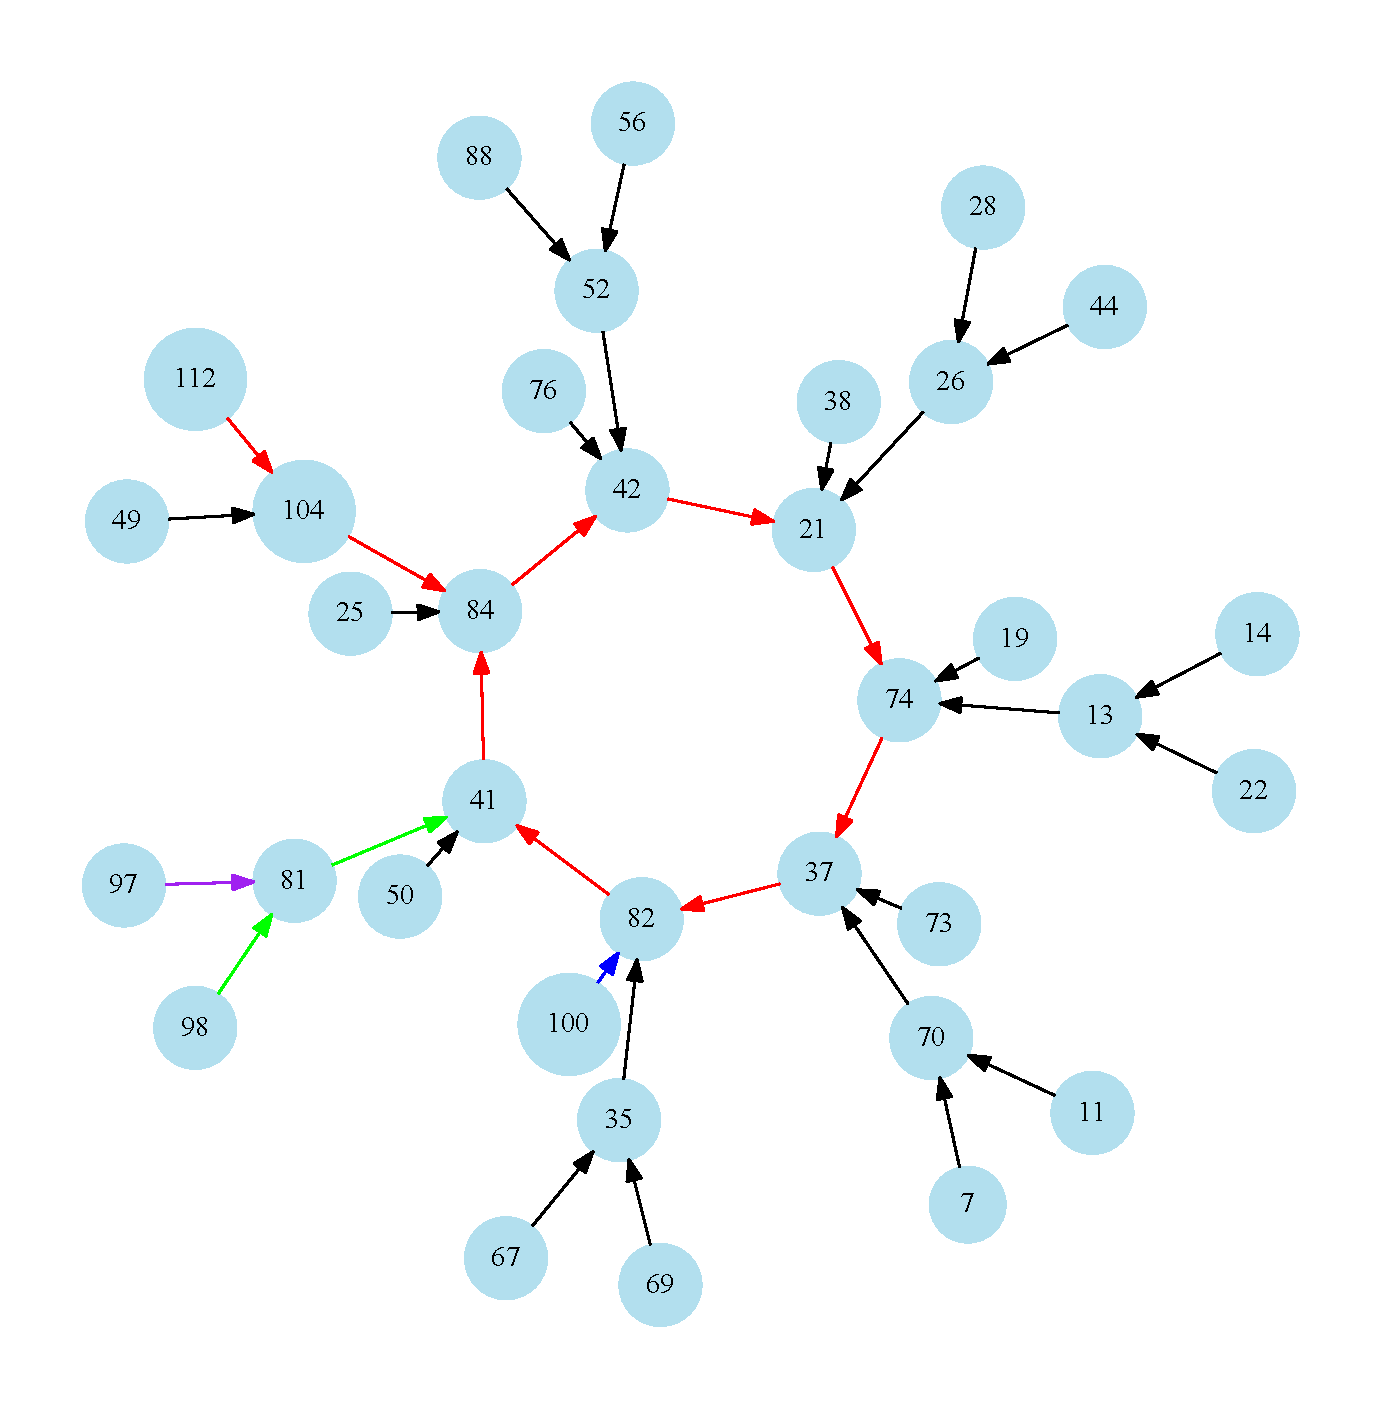
\includegraphics[scale=0.33]{./images/graph5}
\caption{\textcolor{purple}{$13$} premi\`eres it\'erations}
\end{figure}
\end{frame}

\begin{frame}{Algorithme : analyse}
Complexit\'e :
\begin{itemize}
\item calcul des it\'er\'ees de $f$ : $|E|$ ;
\item m\'emoire : $O(|E|)$.
\end{itemize}
Avantages :
\begin{itemize}
\item r\'esultat pouvant \^etre organis\'e en composantes connexes;
\item r\'esultat r\'esum\'e sous forme de chemins et de circuits.
\end{itemize}
Inconv\'enient : n\'ecessite une structure de donn\'ees bien con\c cue.
\end{frame}

\begin{frame}{Am\'elioration de l'algorithme}{Complexit\'e m\'emoire}
Soit $k\in [\![0, n]\!]$. On note $E_{k}\subset E$ l'ensemble des entiers ayant $k$ 1 dans leur \'ecriture en base $2$. Alors : \[f(E_{k})\subset E_k\]

$\Longrightarrow$ nouvelle complexit\'e m\'emoire : $O(C^{n/2}_{n})=O(\frac{|E|}{\sqrt{n}})$.\par

\vspace*{1cm}

Application num\'erique : \[\frac{2^{20}}{C^{10}_{20}}\approx 0,176\]

\end{frame}

\begin{frame}{Am\'elioration de l'algorithme}{Sym\'etrie}
\begin{thm}
Soient $F_1$ et $F_2$ deux parties de $E$ stables par $f$. On note $f_{1}=f_{|F_{1}}$ et $f_{2}=f_{|F_{2}}$. Alors $G_{f_1}\equiv G_{f_2}$ si et seulement s'il existe $\phi:F_{1}\rightarrow F_{2}$ bijective qui commute avec $f$.
\end{thm}
\end{frame}

\begin{frame}{Sym\'etrie}{Applications}
On pose :
\begin{itemize}
\item $I:E\rightarrow E$ l'inversion bit-\`a-bit ;
\item $S:E\rightarrow E$ la sym\'etrie ;
\item $D:E\rightarrow E$ le d\'ecalage des chiffres vers la droite.
\end{itemize}
Alors on peut appliquer le th\'eor\`eme pr\'ec\'edent aux objets :
\begin{itemize}
\item $F_{1}=E_{k}$, $F_{2}=E_{n-k}$ et $\phi=S\circ I$ ;
\item $F_{1}$, $F_{2}$ deux arborescences adjacentes attach\'ees \`a une m\^eme composante connexe et $\phi=D$.
\end{itemize}
On obtient respectivement :
\begin{itemize}
\item $G_{f_{|E_{k}}}\equiv G_{f_{|E_{n-k}}}$ ;
\item l'homog\'en\'eit\'e des composantes connexes.
\end{itemize}
\end{frame}

\begin{frame}
\begin{figure}
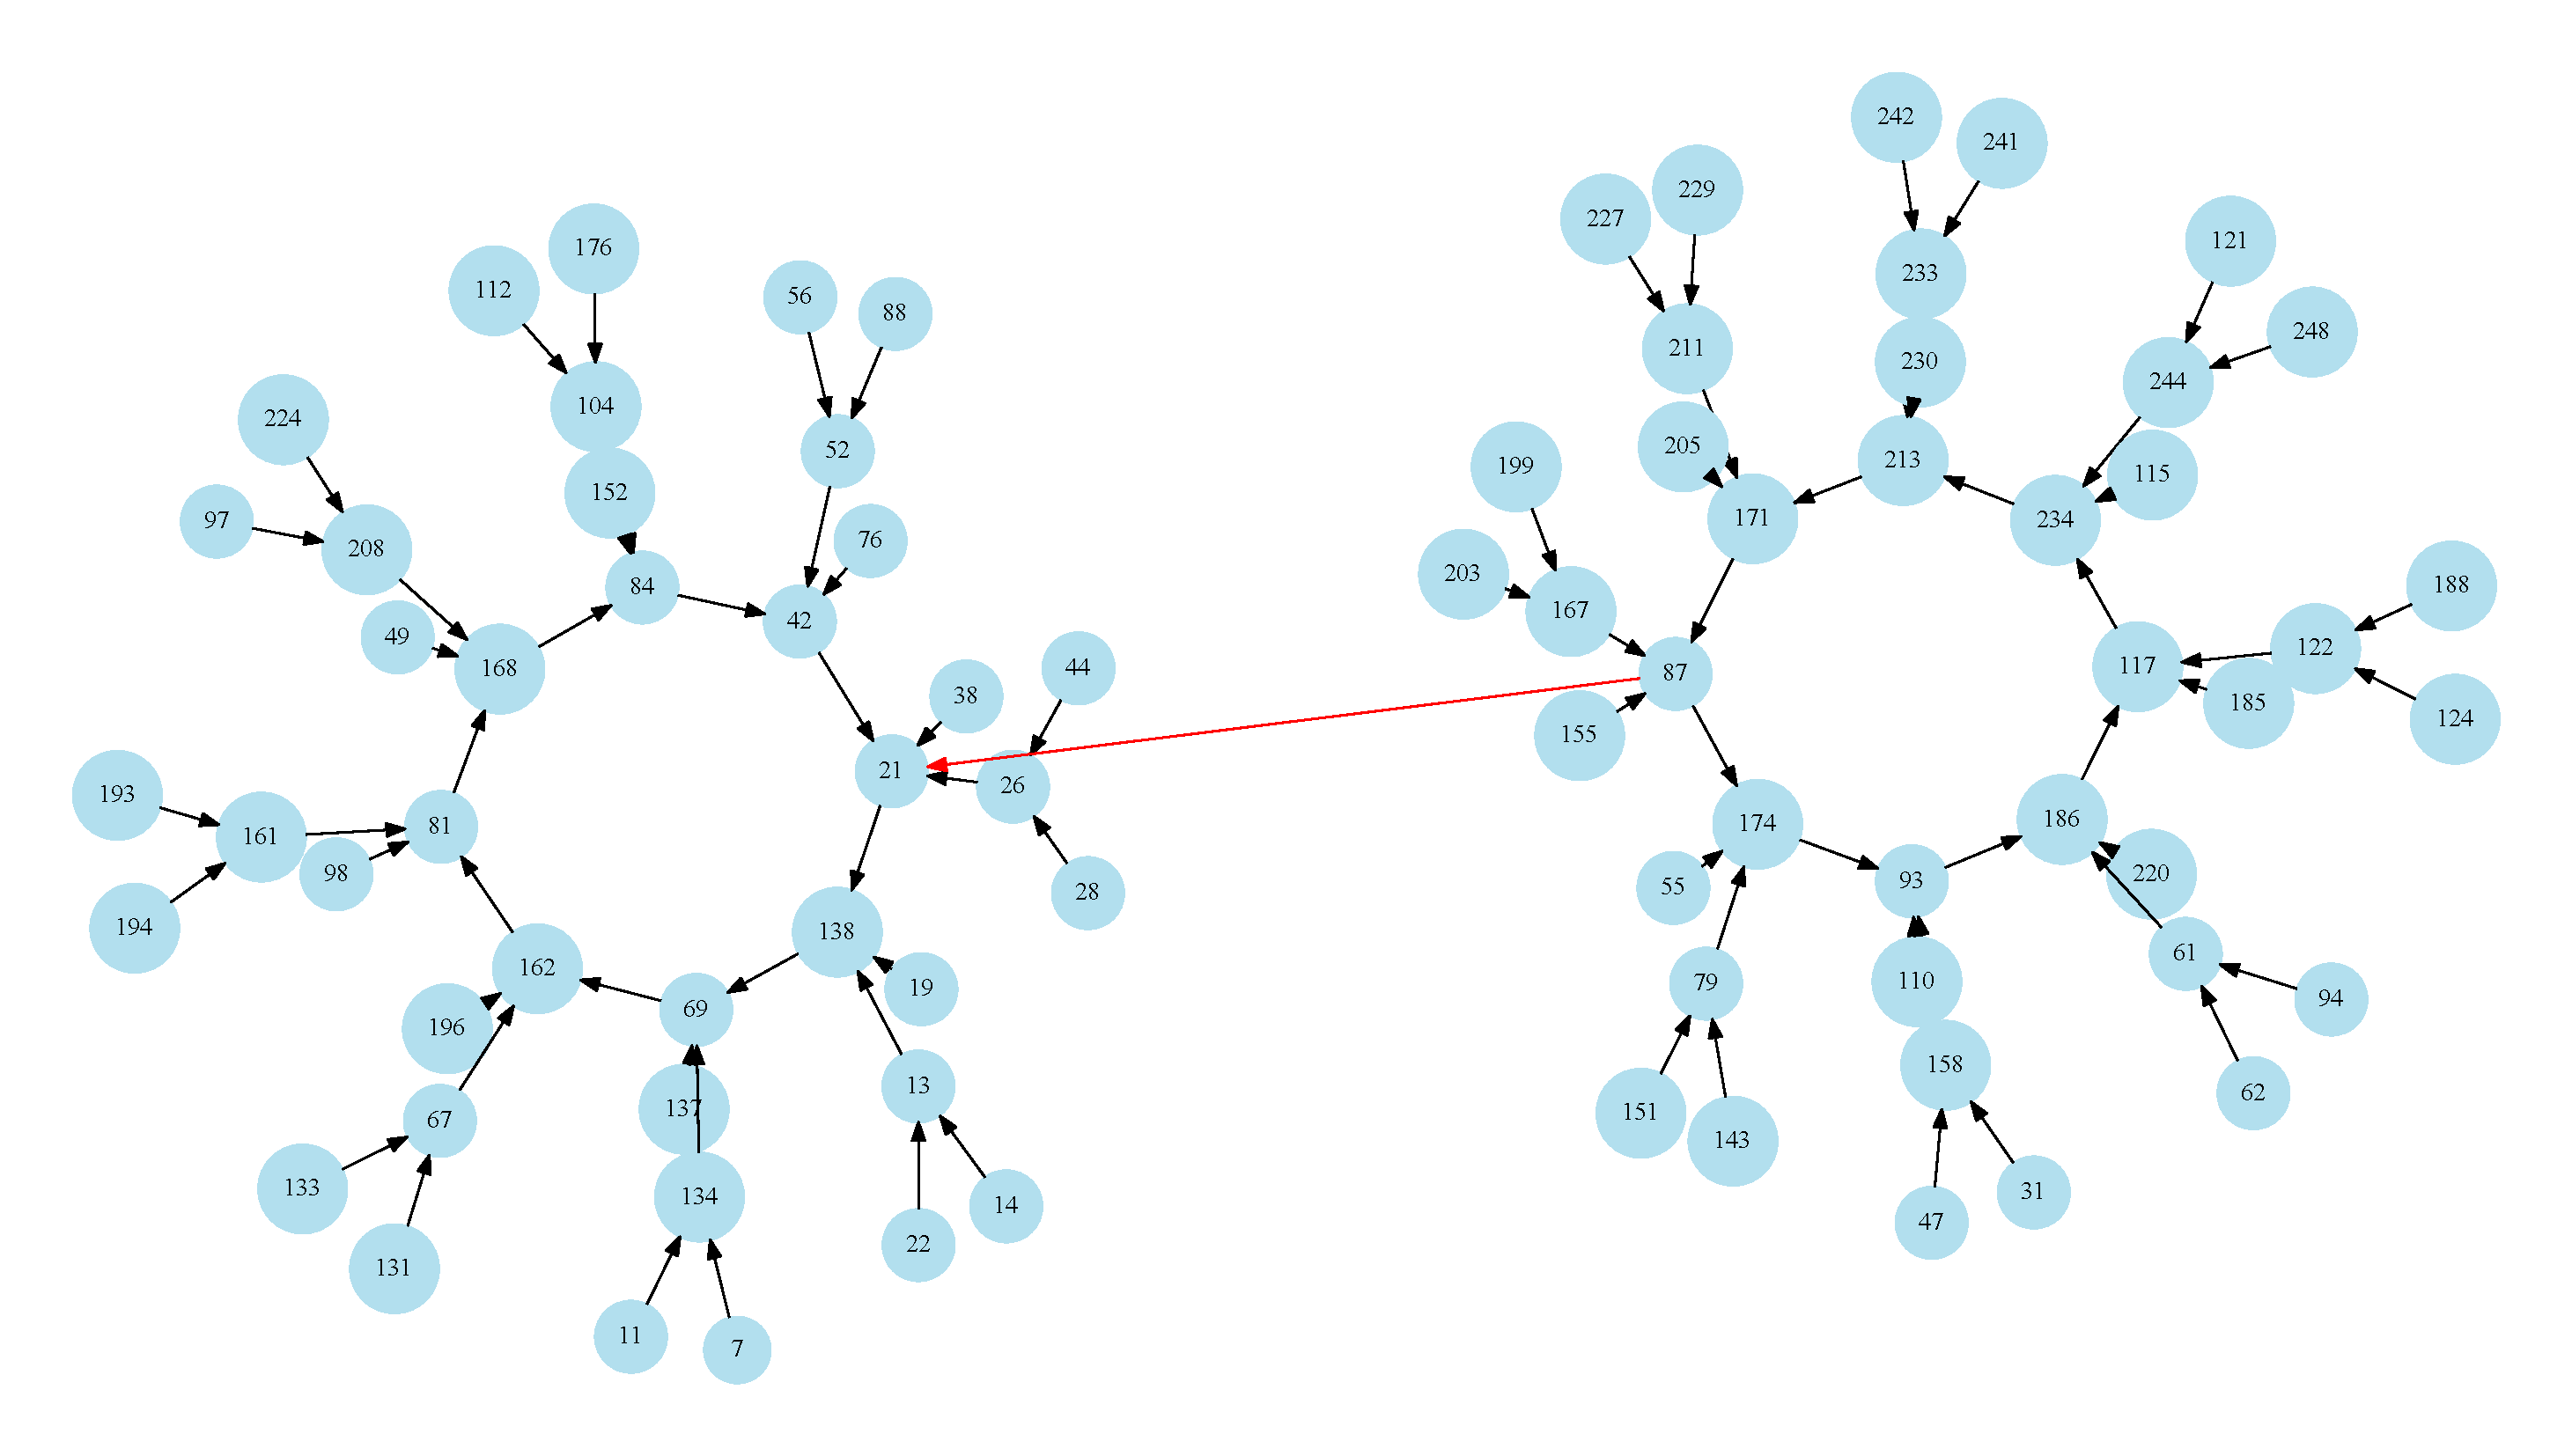
\includegraphics[scale=0.25]{./images/graph_sym1}
\caption{deux composantes connexes de $G_f$ pour $n=8$ et $k=3$, li\'ees par \color{red}{$\phi=S\circ I$}}
\end{figure}
\end{frame}

\begin{frame}
\begin{figure}
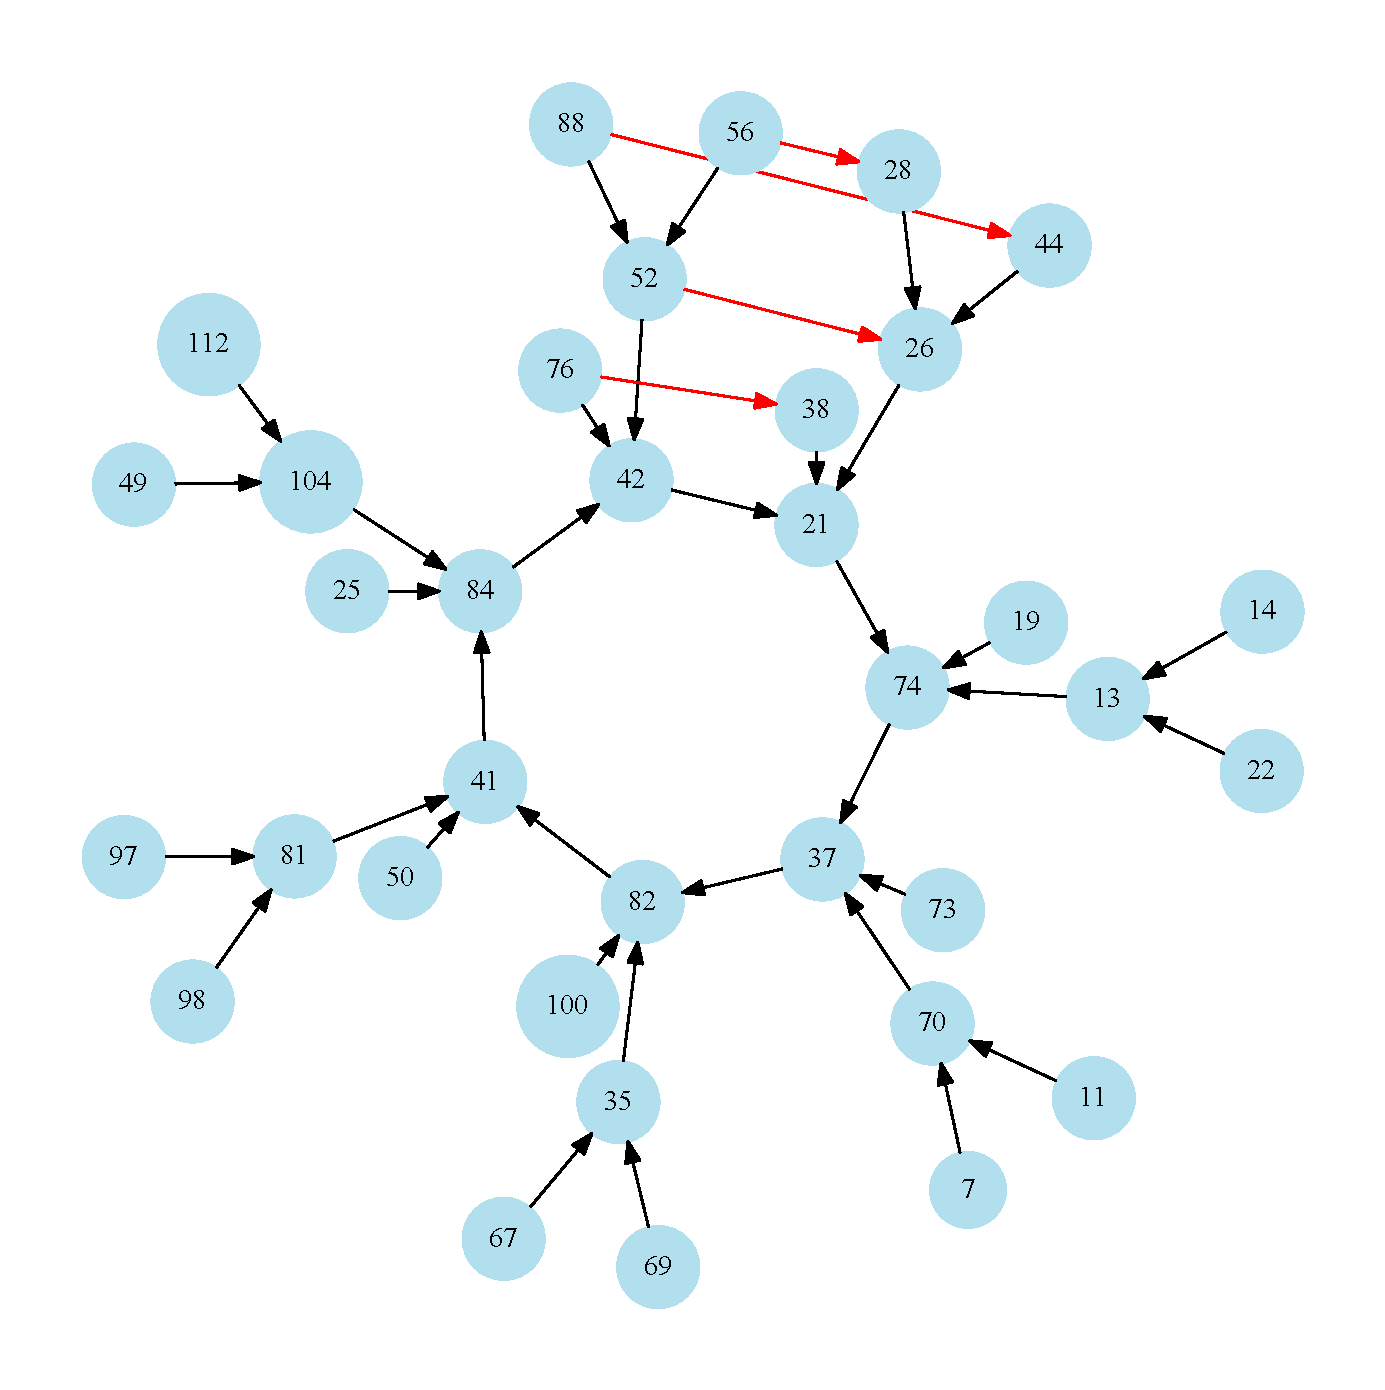
\includegraphics[scale=0.3]{./images/graph_7_3_1_mod}
\caption{une composante connexe de $G_f$ pour $n=7$ et lien avec \color{red}{$\phi=D$}}
\end{figure}
\end{frame}

\subsection{Observations}
\begin{frame}{Observations}
\begin{dftn}
On note \csg{p}{$\sum \mathcal{T}_k$} le circuit de longueur $p$ dont chaque sommet est racine d'une arborescence dont les sous-arborescences sont les $\mathcal{T}_k$. On d\'efinit aussi quatre arborescences not\'ees $\mathcal{T}_1$, $\mathcal{T}_2$, $\mathcal{T}_3$ et $\mathcal{T}_4$, visibles ci-apr\`es.
\end{dftn}
\end{frame}

\begin{frame}
\begin{figure}
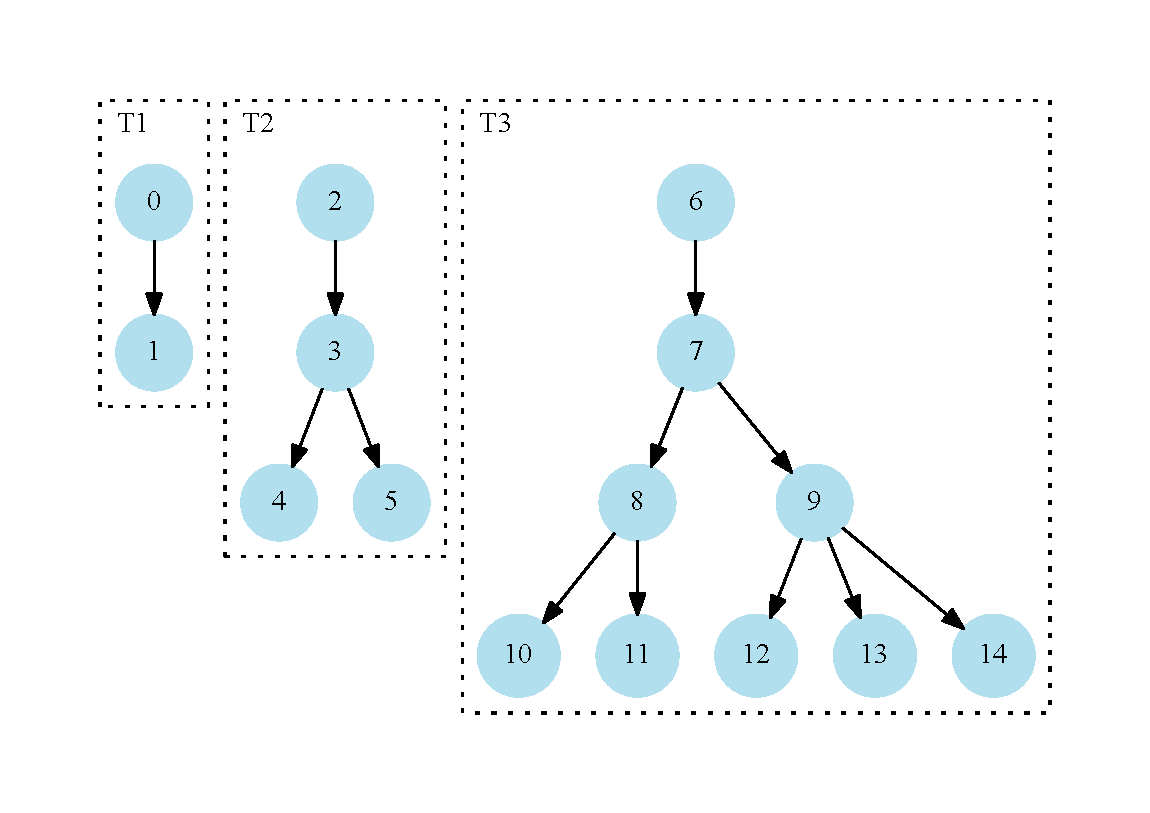
\includegraphics[scale=0.5]{./images/t1_2_3}
\caption{$\mathcal{T}_1$, $\mathcal{T}_2$ et $\mathcal{T}_3$}
\end{figure}
\end{frame}

\begin{frame}
\begin{figure}
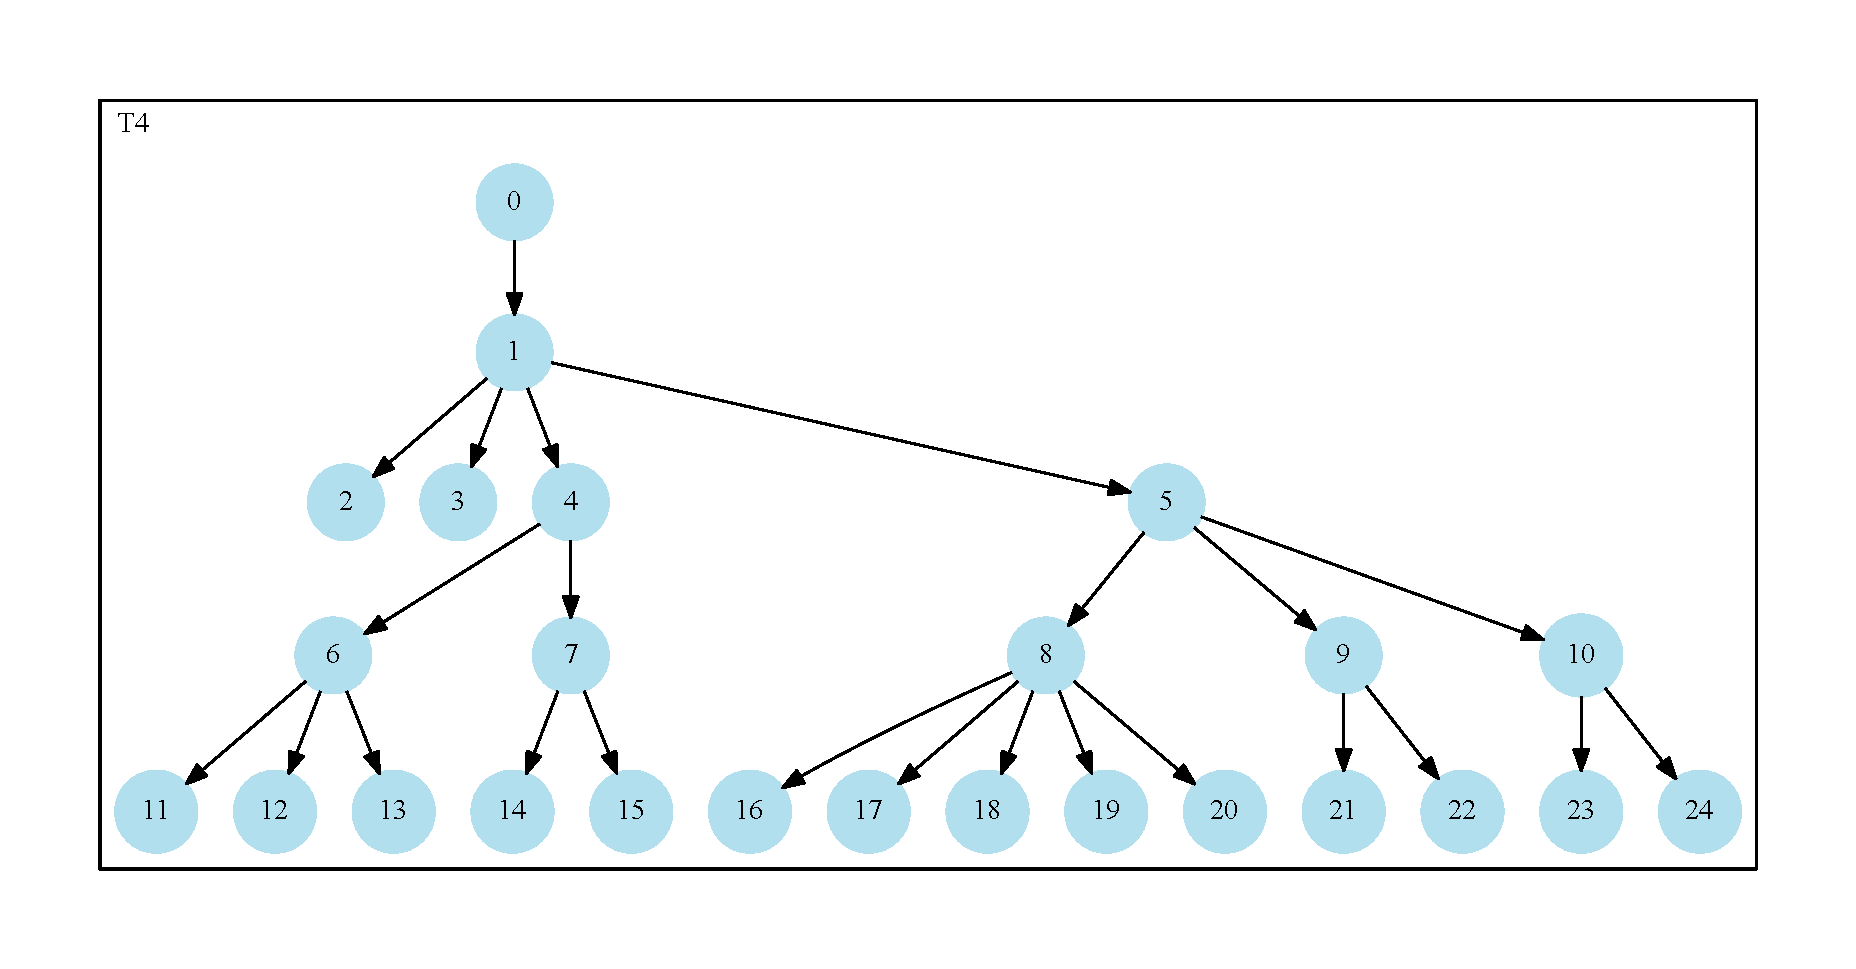
\includegraphics[scale=0.4]{./images/t4}
\caption{$\mathcal{T}_4$}
\end{figure}
\end{frame}

\begin{frame}{R\'esultats}
\begin{figure}
\begin{center}
\begin{tabular}{|c||c|}\hline
$n$ & graphes\\\hline
2 & 2\cycle{1} \cycle{2}\\\hline
3 & 2\cycle{1} 2\cycle{3}\\\hline
4 & 2\cycle{1} 2\cycle{4} \csg{2}{$2\mathcal{T}_{1}$}\\\hline
5 & 2\cycle{1} 2\cycle{5} 2\csg{5}{$\mathcal{T}_{1}$}\\\hline
6 & 2\cycle{1} 2\cycle{3} 2\cycle{6} 2\csg{6}{$\mathcal{T}_{1}$} \csg{2}{$\mathcal{T}_{2}$}\\\hline
7 & 2\cycle{1} 2\cycle{7} 2\csg{7}{$\mathcal{T}_{1}$} 2\csg{7}{$\mathcal{T}_{1}+\mathcal{T}_{2}$}\\\hline
8 & 2\cycle{1} 2\cycle{4} 4\cycle{8} 4\csg{8}{$\mathcal{T}_{1}$} 2\csg{8}{$\mathcal{T}_{1}+\mathcal{T}_{2}$} \csg{2}{$2\mathcal{T}_{1}+4\mathcal{T}_{3}$}\\\hline
9 & 2\cycle{1} 2\cycle{3} 6\cycle{9} 6\csg{9}{$\mathcal{T}_{1}$} 2\csg{9}{$\mathcal{T}_{1}+\mathcal{T}_{2}$} 2\csg{9}{$2\mathcal{T}_{1}+\mathcal{T}_{2}+\mathcal{T}_{3}$}\\\hline
10 & 2\cycle{1} 2\cycle{5} 2\csg{5}{$3\mathcal{T}_{1}$} 8\cycle{10} 8\csg{10}{$\mathcal{T}_{1}$} 4\csg{10}{$\mathcal{T}_{1}+\mathcal{T}_{2}$}\\
& 2\csg{10}{$2\mathcal{T}_{1}+\mathcal{T}_{2}+\mathcal{T}_{3}$} \csg{2}{$5\mathcal{T}_{1}+5\mathcal{T}_{4}$}\\\hline
\end{tabular}
\end{center}
\caption{graphe de $f$ en fonction de $n$}
\end{figure}
\end{frame}